\section{Sample 02: Belief propagation, part A}

The aim of this series of examples is to show how to perform probabilistic queries on factor graphs.

\subsection{part 01}

\begin{figure}
\begin{tabular}{cc}
\begin{minipage}[t]{0.25 \columnwidth}
	\centering
\def\svgwidth{0.9 \textwidth}
\import{../Chapter_additional/04_Samples/image_02/}{graph_1.pdf_tex} 
\end{minipage} 
 & 
\begin{minipage}[t]{0.48 \columnwidth}
\begin{tabular}{|l|l|l|}
$A$ & $B$ & $\Psi_{AB}(A,B) = E(A,B)$ \\
\hline
0 & 0 & exp(w) \\
\hline
0 & 1 & 1 \\
\hline
1 & 0 & 1 \\
\hline
1 & 1 & exp(w) \\
\hline
\end{tabular}
\end{minipage} 
\end{tabular}
\caption{On the left the graph considered in this example, while on the right the image of factor $\Psi_{AB}$. Since that potential is the only one present in the graph, the values in the image of $\Psi_{AB}$ are also the ones assume by the energy function $E$.}
\label{fig:sample_02:0}
\end{figure}

This example creates a graph having a single binary exponential shape $\Psi_{AB}$, see Figure \ref{fig:sample_02:0}, with a $A$ and $B$ having a $Dom$ size equal to 2.  
$\Psi_{AB} = exp(w \Phi_{AB})$, where $\Phi_{AB}$ is a simple correlating factor. The image of $\Psi_{AB}$ is reported in the right part of Figure \ref{fig:sample_02:0}.
\\
Variable $B$ is considered as an evidence, whose value is equal, for the first part of the example, to 0, while a value of 1 is assumed in the second part.
The probability of $A$ conditioned to $B$, is equal to (see equation (\ref{eq:00:cond_prob})):
\begin{eqnarray}
\mathbb{P}(A = a | B = 0) = \frac{E(A = a, B = 0)}{E(A = 0, B = 0) + E(A = 1, B = 0)} 
\Rightarrow \begin{bmatrix}
\mathbb{P}(A = 0 | B = 0) = \frac{exp(w)}{1 + exp(w)}
\\ 
\mathbb{P}(A = 1 | B = 0) = \frac{1}{1 + exp(w)}
\end{bmatrix}
 \\
\mathbb{P}(A = a | B = 1) = \frac{E(A = a, B = 1)}{E(A = 0, B = 1) + E(A = 1, B = 1)} 
\Rightarrow \begin{bmatrix}
\mathbb{P}(A = 0 | B = 1) = \frac{1}{1 + exp(w)}
\\ 
\mathbb{P}(A = 1 | B = 1) = \frac{exp(w)}{1 + exp(w)}
\end{bmatrix}
\end{eqnarray}

\subsection{part 02}

\begin{figure}
\begin{tabular}{ccc}
\begin{minipage}[t]{0.25 \columnwidth}
	\centering
\def\svgwidth{0.9 \textwidth}
\import{../Chapter_additional/04_Samples/image_02/}{graph_2_a.pdf_tex} 
\end{minipage} 
 & 
\begin{minipage}[t]{0.3 \columnwidth}
\begin{tabular}{|l|l|l|}
$A$ & $B$ & $\Psi_{AB}(A,B)$ \\
\hline
0 & 0 & exp($\beta$) \\
\hline
0 & 1 & 1 \\
\hline
1 & 0 & 1 \\
\hline
1 & 1 & exp($\beta$) \\
\hline
\end{tabular}
\end{minipage} 
 & 
\begin{minipage}[t]{0.3 \columnwidth}
\begin{tabular}{|l|l|l|}
$B$ & $C$ & $\Psi_{BC}(B,C)$ \\
\hline
0 & 0 & exp($\alpha$) \\
\hline
0 & 1 & 1 \\
\hline
1 & 0 & 1 \\
\hline
1 & 1 & exp($\alpha$) \\
\hline
\end{tabular}
\end{minipage} 
\end{tabular}
\caption{On the left the graph considered in this example, while on the right the images of factor $\Psi_{AB}$ and $\Psi_{BC}$ having, respectively, a weight equal to $\beta$  and $\alpha$. }
\label{fig:sample_02:1}
\end{figure}

\begin{figure}
	\centering
\def\svgwidth{0.65 \textwidth}
\import{../Chapter_additional/04_Samples/image_02/}{graph_2.pdf_tex} 
\caption{Belief propagation steps when $C$ is assumed as evidence.}
\label{fig:sample_02:2}
\end{figure}

\begin{figure}
	\centering
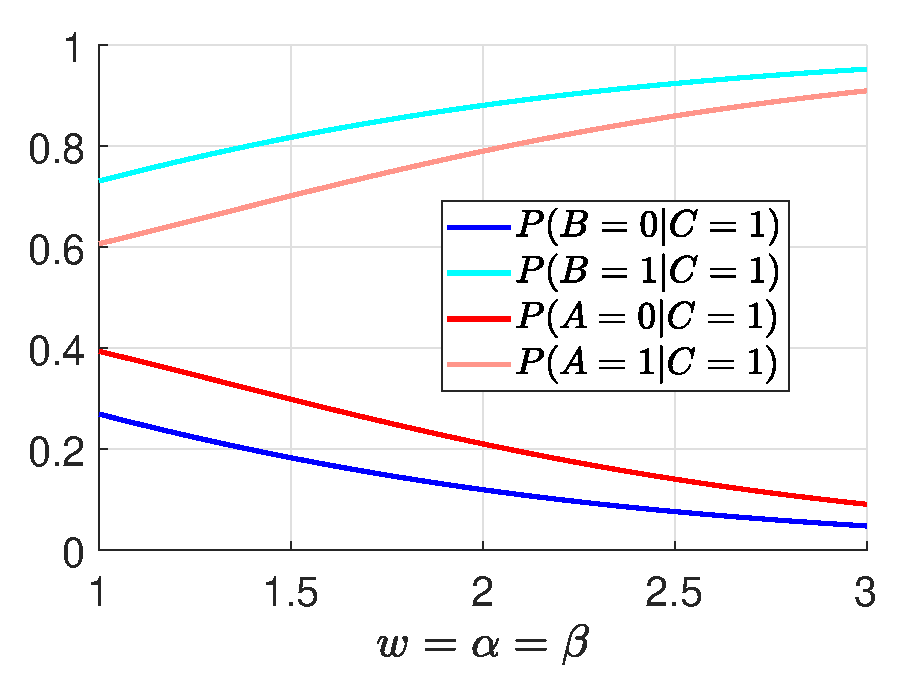
\includegraphics[width=0.48\columnwidth]{../Chapter_additional/04_Samples/image_02/chain_corr.eps}
\caption{The marginals of variables $B$ and $A$, when having a $C=1$ as evidence of the graph reported in Figure \ref{fig:sample_02:2}.}
\label{fig:sample_02:3}
\end{figure} 

\begin{figure}
	\centering
\def\svgwidth{0.65 \textwidth}
\import{../Chapter_additional/04_Samples/image_02/}{graph_2_b.pdf_tex} 
\caption{Belief propagation steps when $B$ is assumed as evidence.}
\label{fig:sample_02:4}
\end{figure} 

A slightly more complex graph, made of two exponential correlating factors $\Psi_{BC}$ and $\Psi_{AB}$, is built in this sample. The considered graph is reported in Figure \ref{fig:sample_02:1}. The two involved factors have two different weights, $\alpha$ and $\beta$: the resulting image sets are reported in the right part of Figure \ref{fig:sample_02:1}. 
\\
In the first part, $C = 1$ is assumed as evidence and the marginal probabilities of $A$ and $B$ conditioned to $C$ are computed. They are compared with the theoretical results, obtained by applying the message passing algorithm (Section \ref{sec:00:MP}), whose steps are here detailed \footnote{The same steps are internally execute by Node$\_$factory.}. The message passing steps are summarized in Figure \ref{fig:sample_02:2}. After having computed all the messages, it is clear that the marginal probabilities are equal to:
\begin{eqnarray}
\mathbb{P}(A | C = 1) = \frac{1}{Z}   M_{B \rightarrow A}(A) = \frac{1}{Z} \begin{bmatrix} exp(\alpha) + exp(\beta) \\ 1 + exp(\alpha) \cdot exp(\beta)  \end{bmatrix} \\
\mathbb{P}(B | C = 1) = \frac{1}{Z} \Phi_B(B) \cdot M_{A \rightarrow B}(B) = \frac{1}{Z} \Phi_B(B) = \frac{1}{Z} \begin{bmatrix} 1 \\ exp(\alpha)  \end{bmatrix}
\end{eqnarray}
Figure \ref{fig:sample_02:3} shows the values assumed by the marginals when varying the coefficients $\alpha$  and $\beta$. As can be seen, the more $A,B$ and $C$ are correlated (i.e. the more $\alpha$  and $\beta$ are big) the more $\mathbb{P}(B=1|C=1)$ and $\mathbb{P}(A=1|C=1)$ are big. Notice also that when assuming $\alpha=\beta$,  $\mathbb{P}(B=1|C=1)$ is always bigger than $\mathbb{P}(A=1|C=1)$. This is intuitively explained by the fact that $C$ is directly connected to $B$, while $A$ is indirectly connected to $C$, through $B$.
\\
In the second part, $B = 1$ is assumed as evidence and the marginal probabilities of $A$ and $C$ conditioned to $B$ are computed. The theoretical results can be computed again considering the message passing, whoe steps are reported in Figure \ref{fig:sample_02:4}.
The marginal probabilities are in this case equal to:
\begin{eqnarray}
\mathbb{P}(A | B = 1) = \frac{1}{Z}  \Phi_A(A) = \frac{1}{Z}  \begin{bmatrix} 1 \\ exp(\beta)  \end{bmatrix} \\
\mathbb{P}(C | B = 1) = \frac{1}{Z}  \Phi_C(C) = \frac{1}{Z}  \begin{bmatrix} 1 \\ exp(\alpha)  \end{bmatrix} 
\end{eqnarray}


\subsection{part 03}

\begin{figure}
\begin{tabular}{c}
\begin{minipage}[t]{0.8 \columnwidth}
	\centering
\def\svgwidth{0.9 \textwidth}
\import{../Chapter_additional/04_Samples/image_02/}{graph_3.pdf_tex} 
\end{minipage} 
 \\ 
\begin{minipage}[t]{0.39 \columnwidth}
	\centering
\begin{tabular}{l|l|l|l|l|}
 $\Psi_i(Y_{i-1}, Y_i)$ & $Y_i = 0$ & $Y_i = 1$ & $\cdots$ & $Y_i = m$ \\
      \hline
$Y_{i-1} = 0$ 		  & $exp(w)$& $1$     & $\cdots$     & $1$     \\
\hline
$Y_{i-1} = 1$ 		  & $1$     & $exp(w)$& $\cdots$     & $1$    \\
\hline
$\vdots$ 		  		  & $\vdots$     & $\vdots$     & $\ddots$ & $\vdots$   \\
\hline
$Y_{i-1} = m$ 		  & $1$     & $1$     & $\cdots$ & $exp(w)$   \\
\hline 
\end{tabular}
\end{minipage} 
\end{tabular}
\caption{On the top the chain considered in this example, while on the bottom the image of the generic factor $\Psi_i(Y_{i-1}, Y_i)$.}
\label{fig:sample_02:5}
\end{figure}

\begin{figure}
	\centering
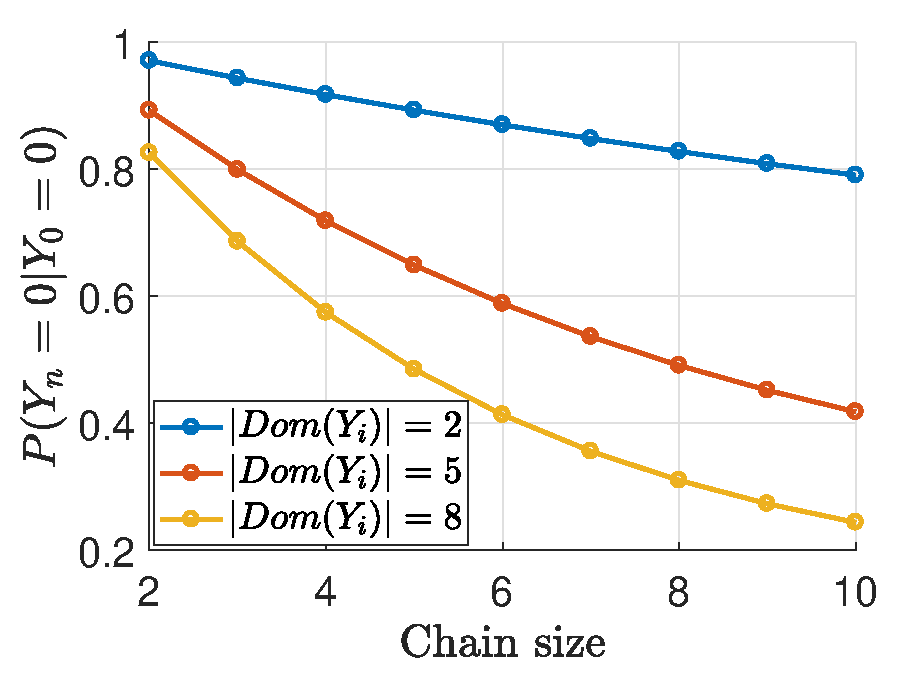
\includegraphics[width=0.48 \columnwidth]{../Chapter_additional/04_Samples/image_02/Chain_marginals.eps}
\caption{Marginal probability of $Y_n$ when varying the chain size of the structure presented in Figure \ref{fig:sample_02:5}. $w$ is assumed equal to $3.5$.}
\label{fig:sample_02:6}
\end{figure} 


In this sample, a linear chain of variables $Y_{0,1,2,\cdots,n}$ is considered. All variables in the chain have the same $Dom$ size and all the factors $\Psi_{1,\cdots,n}$, Figure \ref{fig:sample_02:5}, are simple exponential correlating factors. The image of the generic factor $\Psi_i$ is reported in the right part of Figure \ref{fig:sample_02:5}.
\\
The evidence $Y_0=0$ is assumed and the marginals of the last variable in the chain $Y_n$, i.e. the one furthest to $Y_0$, are computed. Figure \ref{fig:sample_02:6} reports the probability $\mathbb{P}(Y_n = 0 | Y_0 = 0)$, when varying the chain size, as well the domain size of the variables. As can be seen, the more the chain is longer, the lower is the aforementioned probability, as $Y_n$ is more and more indirectly correlated to $Y_0$. Similar considerations hold for the domain size.



